\begin{figure*}[tp]
\centering
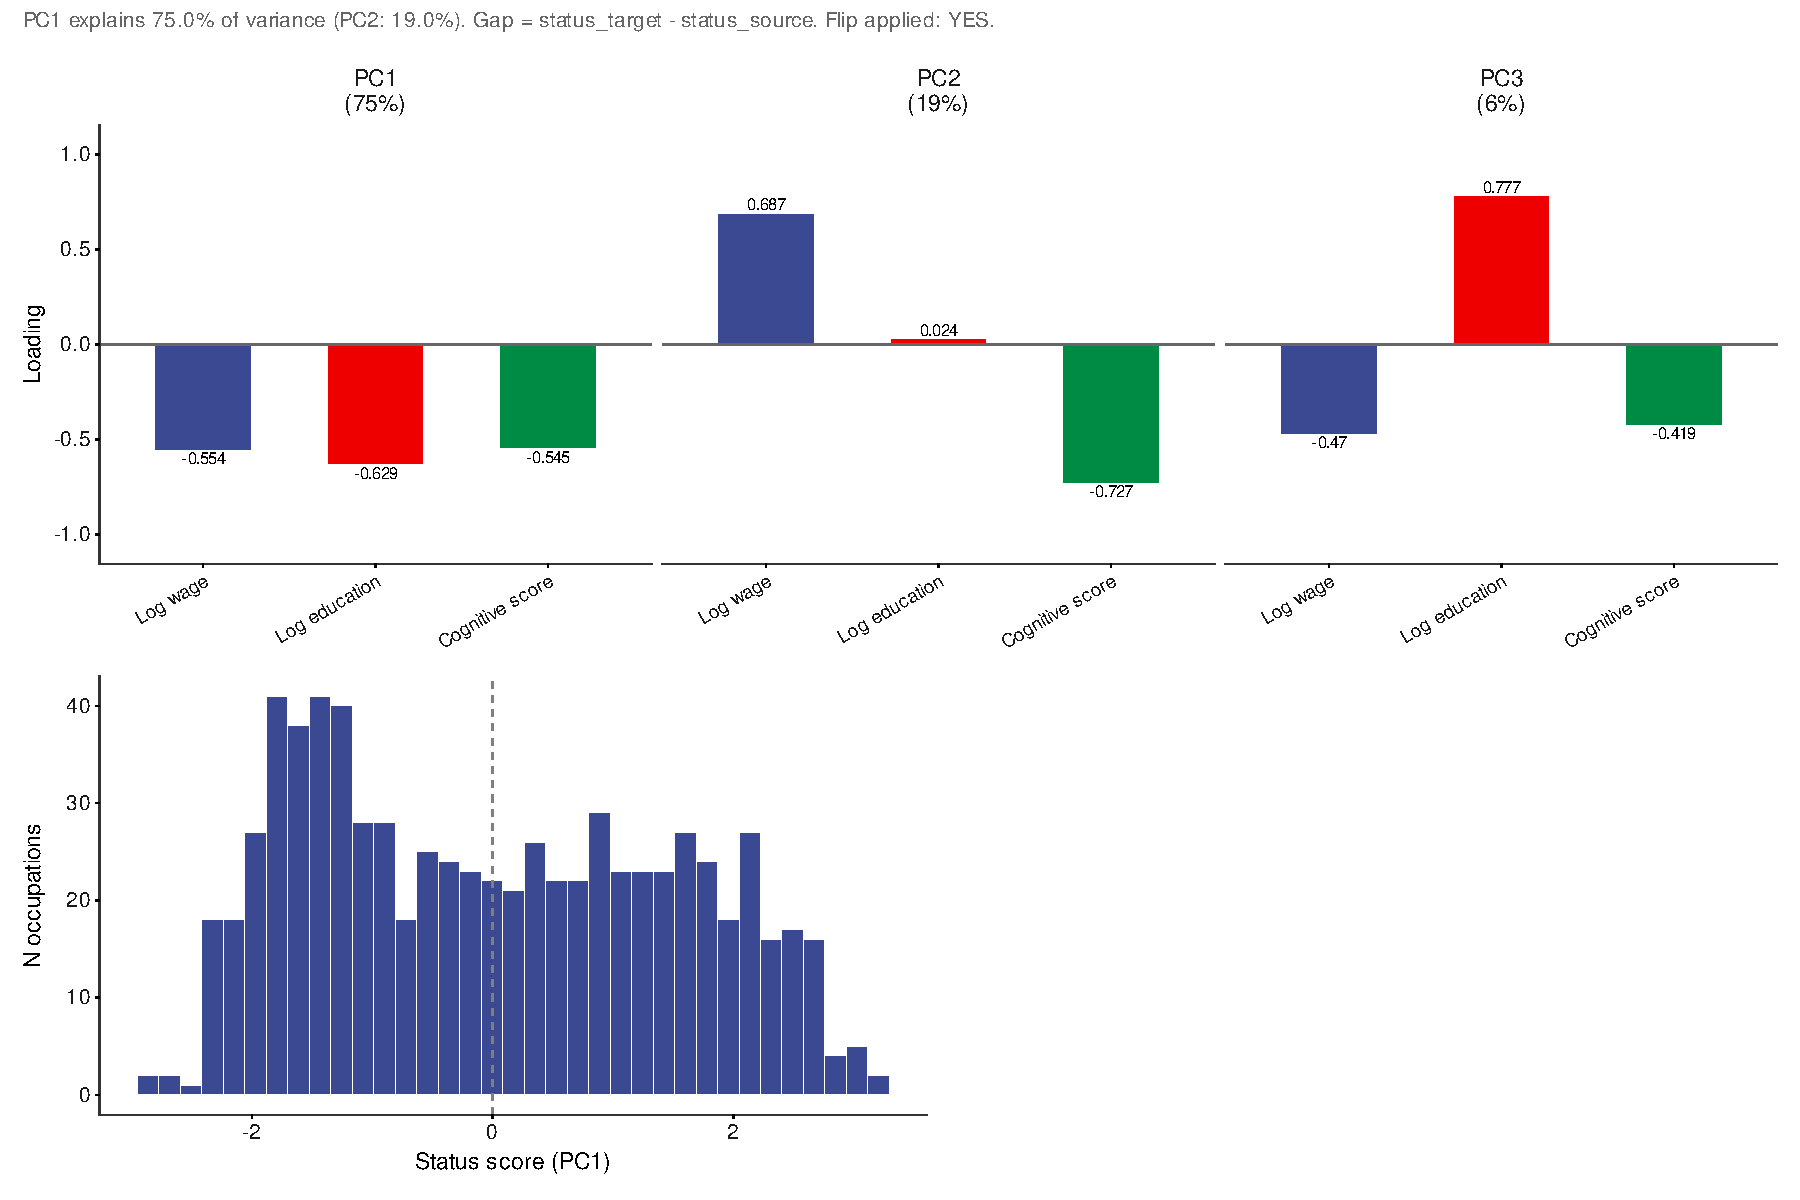
\includegraphics[width=0.95\textwidth]{figures/fig_pca_status.pdf}
\caption{\textbf{Principal component analysis of the occupational status index.}
\textbf{(A)} PCA loadings for the three principal components extracted from log-transformed median wage (BLS OEWS 2015), log-transformed expected level of required education (O*NET Scale RL), and cognitive task content (fraction of O*NET importance weight accounted for by socio-cognitive skill items), estimated with mean-centering and unit-variance scaling across all 741 occupations in the analytic sample. PC1 captures 75.0\% of joint variance, with loadings of comparable magnitude across all three variables (log wage: $|{-}0.554|$; log education: $|{-}0.629|$; cognitive score: $|{-}0.545|$), confirming convergence on a single underlying status axis. The sign of PC1 is reversed (flip applied) so that higher values correspond to higher occupational status. \textbf{(B)} Distribution of occupation-level status scores ($\sigma_i$) across the 741 analytic occupations. The dashed vertical line marks the origin ($\sigma_i = 0$), which corresponds to the sample mean after mean-centering. The signed status gap for each directed dyad is computed as $G_{ij} = \sigma_j - \sigma_i$.}
\label{fig:SI_pca_status}
\end{figure*}
